\documentclass[1p]{elsarticle_modified}
%\bibliographystyle{elsarticle-num}

%\usepackage[colorlinks]{hyperref}
%\usepackage{abbrmath_seonhwa} %\Abb, \Ascr, \Acal ,\Abf, \Afrak
\usepackage{amsfonts}
\usepackage{amssymb}
\usepackage{amsmath}
\usepackage{amsthm}
\usepackage{scalefnt}
\usepackage{amsbsy}
\usepackage{kotex}
\usepackage{caption}
\usepackage{subfig}
\usepackage{color}
\usepackage{graphicx}
\usepackage{xcolor} %% white, black, red, green, blue, cyan, magenta, yellow
\usepackage{float}
\usepackage{setspace}
\usepackage{hyperref}

\usepackage{tikz}
\usetikzlibrary{arrows}

\usepackage{multirow}
\usepackage{array} % fixed length table
\usepackage{hhline}

%%%%%%%%%%%%%%%%%%%%%
\makeatletter
\renewcommand*\env@matrix[1][\arraystretch]{%
	\edef\arraystretch{#1}%
	\hskip -\arraycolsep
	\let\@ifnextchar\new@ifnextchar
	\array{*\c@MaxMatrixCols c}}
\makeatother %https://tex.stackexchange.com/questions/14071/how-can-i-increase-the-line-spacing-in-a-matrix
%%%%%%%%%%%%%%%

\usepackage[normalem]{ulem}

\newcommand{\msout}[1]{\ifmmode\text{\sout{\ensuremath{#1}}}\else\sout{#1}\fi}
%SOURCE: \msout is \stkout macro in https://tex.stackexchange.com/questions/20609/strikeout-in-math-mode

\newcommand{\cancel}[1]{
	\ifmmode
	{\color{red}\msout{#1}}
	\else
	{\color{red}\sout{#1}}
	\fi
}

\newcommand{\add}[1]{
	{\color{blue}\uwave{#1}}
}

\newcommand{\replace}[2]{
	\ifmmode
	{\color{red}\msout{#1}}{\color{blue}\uwave{#2}}
	\else
	{\color{red}\sout{#1}}{\color{blue}\uwave{#2}}
	\fi
}

\newcommand{\Sol}{\mathcal{S}} %segment
\newcommand{\D}{D} %diagram
\newcommand{\A}{\mathcal{A}} %arc


%%%%%%%%%%%%%%%%%%%%%%%%%%%%%5 test

\def\sl{\operatorname{\textup{SL}}(2,\Cbb)}
\def\psl{\operatorname{\textup{PSL}}(2,\Cbb)}
\def\quan{\mkern 1mu \triangleright \mkern 1mu}

\theoremstyle{definition}
\newtheorem{thm}{Theorem}[section]
\newtheorem{prop}[thm]{Proposition}
\newtheorem{lem}[thm]{Lemma}
\newtheorem{ques}[thm]{Question}
\newtheorem{cor}[thm]{Corollary}
\newtheorem{defn}[thm]{Definition}
\newtheorem{exam}[thm]{Example}
\newtheorem{rmk}[thm]{Remark}
\newtheorem{alg}[thm]{Algorithm}

\newcommand{\I}{\sqrt{-1}}
\begin{document}

%\begin{frontmatter}
%
%\title{Boundary parabolic representations of knots up to 8 crossings}
%
%%% Group authors per affiliation:
%\author{Yunhi Cho} 
%\address{Department of Mathematics, University of Seoul, Seoul, Korea}
%\ead{yhcho@uos.ac.kr}
%
%
%\author{Seonhwa Kim} %\fnref{s_kim}}
%\address{Center for Geometry and Physics, Institute for Basic Science, Pohang, 37673, Korea}
%\ead{ryeona17@ibs.re.kr}
%
%\author{Hyuk Kim}
%\address{Department of Mathematical Sciences, Seoul National University, Seoul 08826, Korea}
%\ead{hyukkim@snu.ac.kr}
%
%\author{Seokbeom Yoon}
%\address{Department of Mathematical Sciences, Seoul National University, Seoul, 08826,  Korea}
%\ead{sbyoon15@snu.ac.kr}
%
%\begin{abstract}
%We find all boundary parabolic representation of knots up to 8 crossings.
%
%\end{abstract}
%\begin{keyword}
%    \MSC[2010] 57M25 
%\end{keyword}
%
%\end{frontmatter}

%\linenumbers
%\tableofcontents
%
\newcommand\colored[1]{\textcolor{white}{\rule[-0.35ex]{0.8em}{1.4ex}}\kern-0.8em\color{red} #1}%
%\newcommand\colored[1]{\textcolor{white}{ #1}\kern-2.17ex	\textcolor{white}{ #1}\kern-1.81ex	\textcolor{white}{ #1}\kern-2.15ex\color{red}#1	}

{\Large $\underline{10_{38}~(K10a_{29})}$}

\setlength{\tabcolsep}{10pt}
\renewcommand{\arraystretch}{1.6}
\vspace{1cm}\begin{tabular}{m{100pt}>{\centering\arraybackslash}m{274pt}}
\multirow{5}{120pt}{
	\centering
	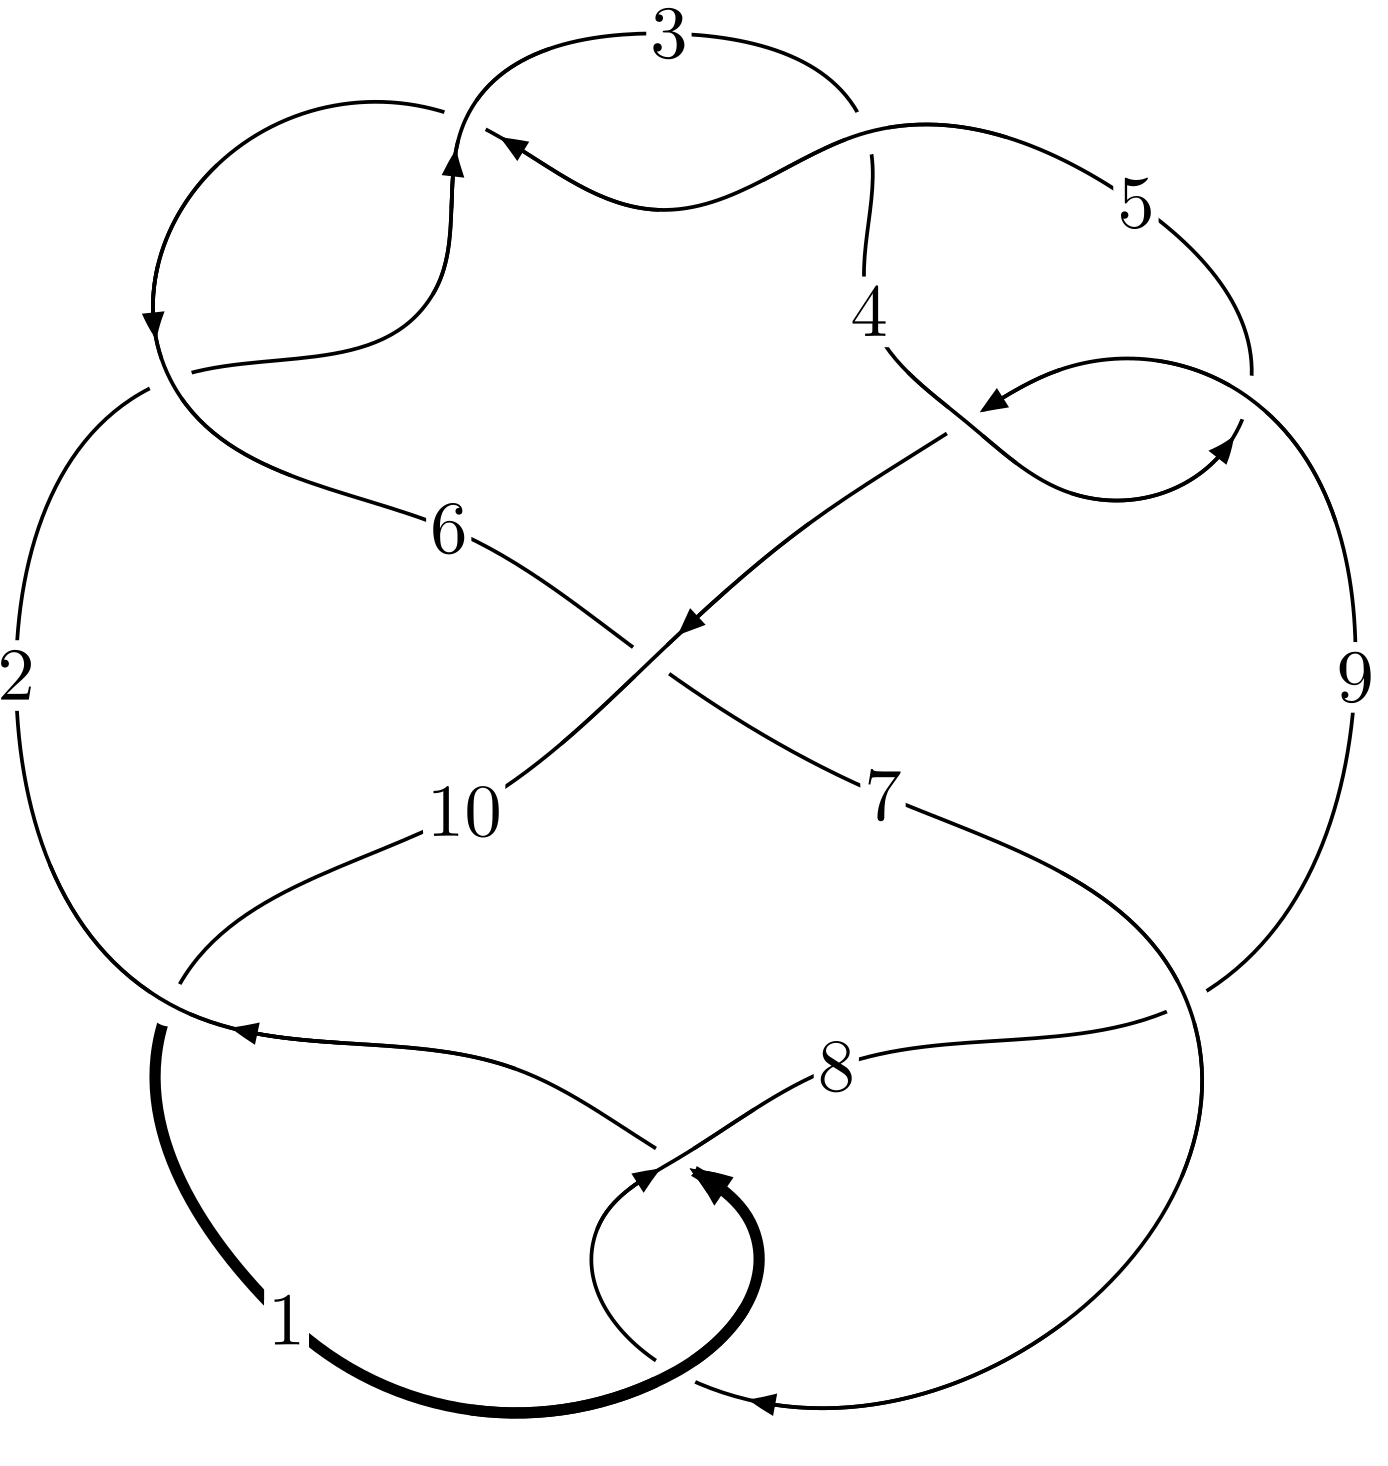
\includegraphics[width=112pt]{../../../GIT/diagram.site/Diagrams/png/122_10_38.png}\\
\ \ \ A knot diagram\footnotemark}&
\allowdisplaybreaks
\textbf{Linearized knot diagam} \\
\cline{2-2}
 &
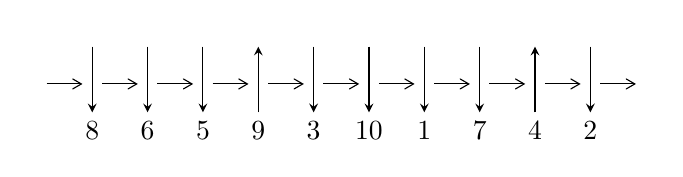
\begin{tikzpicture}[x=20pt, y=17pt]
	% nodes
	\node (C0) at (0, 0) {};
	\node (C1) at (1, 0) {};
	\node (C1U) at (1, +1) {};
	\node (C1D) at (1, -1) {8};

	\node (C2) at (2, 0) {};
	\node (C2U) at (2, +1) {};
	\node (C2D) at (2, -1) {6};

	\node (C3) at (3, 0) {};
	\node (C3U) at (3, +1) {};
	\node (C3D) at (3, -1) {5};

	\node (C4) at (4, 0) {};
	\node (C4U) at (4, +1) {};
	\node (C4D) at (4, -1) {9};

	\node (C5) at (5, 0) {};
	\node (C5U) at (5, +1) {};
	\node (C5D) at (5, -1) {3};

	\node (C6) at (6, 0) {};
	\node (C6U) at (6, +1) {};
	\node (C6D) at (6, -1) {10};

	\node (C7) at (7, 0) {};
	\node (C7U) at (7, +1) {};
	\node (C7D) at (7, -1) {1};

	\node (C8) at (8, 0) {};
	\node (C8U) at (8, +1) {};
	\node (C8D) at (8, -1) {7};

	\node (C9) at (9, 0) {};
	\node (C9U) at (9, +1) {};
	\node (C9D) at (9, -1) {4};

	\node (C10) at (10, 0) {};
	\node (C10U) at (10, +1) {};
	\node (C10D) at (10, -1) {2};
	\node (C11) at (11, 0) {};

	% arrows
	\draw[->,>={angle 60}]
	(C0) edge (C1) (C1) edge (C2) (C2) edge (C3) (C3) edge (C4) (C4) edge (C5) (C5) edge (C6) (C6) edge (C7) (C7) edge (C8) (C8) edge (C9) (C9) edge (C10) (C10) edge (C11) ;	\draw[->,>=stealth]
	(C1U) edge (C1D) (C2U) edge (C2D) (C3U) edge (C3D) (C4D) edge (C4U) (C5U) edge (C5D) (C6U) edge (C6D) (C7U) edge (C7D) (C8U) edge (C8D) (C9D) edge (C9U) (C10U) edge (C10D) ;
	\end{tikzpicture} \\
\hhline{~~} \\& 
\textbf{Solving Sequence} \\ \cline{2-2} 
 &
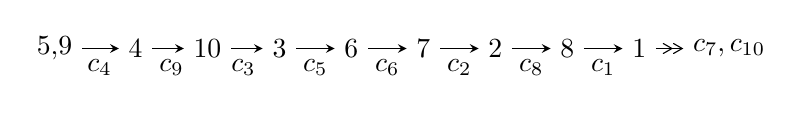
\begin{tikzpicture}[x=26pt, y=7pt]
	% node
	\node (A0) at (-1/8, 0) {5,9};
	\node (A1) at (1, 0) {4};
	\node (A2) at (2, 0) {10};
	\node (A3) at (3, 0) {3};
	\node (A4) at (4, 0) {6};
	\node (A5) at (5, 0) {7};
	\node (A6) at (6, 0) {2};
	\node (A7) at (7, 0) {8};
	\node (A8) at (8, 0) {1};
	\node (C1) at (1/2, -1) {$c_{4}$};
	\node (C2) at (3/2, -1) {$c_{9}$};
	\node (C3) at (5/2, -1) {$c_{3}$};
	\node (C4) at (7/2, -1) {$c_{5}$};
	\node (C5) at (9/2, -1) {$c_{6}$};
	\node (C6) at (11/2, -1) {$c_{2}$};
	\node (C7) at (13/2, -1) {$c_{8}$};
	\node (C8) at (15/2, -1) {$c_{1}$};
	\node (A9) at (37/4, 0) {$c_{7},c_{10}$};

	% edge
	\draw[->,>=stealth]	
	(A0) edge (A1) (A1) edge (A2) (A2) edge (A3) (A3) edge (A4) (A4) edge (A5) (A5) edge (A6) (A6) edge (A7) (A7) edge (A8) ;
	\draw[->>,>={angle 60}]	
	(A8) edge (A9);
\end{tikzpicture} \\ 

\end{tabular} \\

\footnotetext{
The image of knot diagram is generated by the software ``\textbf{Draw programme}" developed by Andrew Bartholomew(\url{http://www.layer8.co.uk/maths/draw/index.htm\#Running-draw}), where we modified some parts for our purpose(\url{https://github.com/CATsTAILs/LinksPainter}).
}\phantom \\ \newline 
\centering \textbf{Ideals for irreducible components\footnotemark of $X_{\text{par}}$} 
 
\begin{align*}
I^u_{1}&=\langle 
u^{29}- u^{28}+\cdots+u+1\rangle \\
\\
\end{align*}
\raggedright * 1 irreducible components of $\dim_{\mathbb{C}}=0$, with total 29 representations.\\
\footnotetext{All coefficients of polynomials are rational numbers. But the coefficients are sometimes approximated in decimal forms when there is not enough margin.}
\newpage
\renewcommand{\arraystretch}{1}
\centering \section*{I. $I^u_{1}= \langle u^{29}- u^{28}+\cdots+u+1 \rangle$}
\flushleft \textbf{(i) Arc colorings}\\
\begin{tabular}{m{7pt} m{180pt} m{7pt} m{180pt} }
\flushright $a_{5}=$&$\begin{pmatrix}1\\0\end{pmatrix}$ \\
\flushright $a_{9}=$&$\begin{pmatrix}0\\u\end{pmatrix}$ \\
\flushright $a_{4}=$&$\begin{pmatrix}1\\u^2\end{pmatrix}$ \\
\flushright $a_{10}=$&$\begin{pmatrix}u\\u^3+u\end{pmatrix}$ \\
\flushright $a_{3}=$&$\begin{pmatrix}u^2+1\\u^2\end{pmatrix}$ \\
\flushright $a_{6}=$&$\begin{pmatrix}u^4+u^2+1\\u^4\end{pmatrix}$ \\
\flushright $a_{7}=$&$\begin{pmatrix}u^8+u^6+3 u^4+2 u^2+1\\u^{10}+2 u^8+3 u^6+4 u^4+u^2\end{pmatrix}$ \\
\flushright $a_{2}=$&$\begin{pmatrix}u^6+u^4+2 u^2+1\\u^6+u^2\end{pmatrix}$ \\
\flushright $a_{8}=$&$\begin{pmatrix}u^{17}+2 u^{15}+7 u^{13}+10 u^{11}+15 u^9+14 u^7+10 u^5+4 u^3+u\\u^{19}+3 u^{17}+8 u^{15}+15 u^{13}+19 u^{11}+21 u^9+14 u^7+6 u^5+u^3+u\end{pmatrix}$ \\
\flushright $a_{1}=$&$\begin{pmatrix}- u^{15}-2 u^{13}-6 u^{11}-8 u^9-10 u^7-8 u^5-4 u^3\\- u^{15}- u^{13}-4 u^{11}-3 u^9-4 u^7-2 u^5+u\end{pmatrix}$\\&\end{tabular}
\flushleft \textbf{(ii) Obstruction class $= -1$}\\~\\
\flushleft \textbf{(iii) Cusp Shapes $= -4 u^{28}-12 u^{26}-4 u^{25}-48 u^{24}-12 u^{23}-100 u^{22}-44 u^{21}-208 u^{20}-92 u^{19}-312 u^{18}-172 u^{17}-424 u^{16}-252 u^{15}-456 u^{14}-296 u^{13}-432 u^{12}-288 u^{11}-328 u^{10}-216 u^9-216 u^8-128 u^7-120 u^6-56 u^5-48 u^4-32 u^3-16 u^2-12 u-10$}\\~\\
\newpage\renewcommand{\arraystretch}{1}
\flushleft \textbf{(iv) u-Polynomials at the component}\newline \\
\begin{tabular}{m{50pt}|m{274pt}}
Crossings & \hspace{64pt}u-Polynomials at each crossing \\
\hline $$\begin{aligned}c_{1},c_{7}\end{aligned}$$&$\begin{aligned}
&u^{29}+u^{28}+\cdots+3 u+1
\end{aligned}$\\
\hline $$\begin{aligned}c_{2},c_{3},c_{5}\end{aligned}$$&$\begin{aligned}
&u^{29}+7 u^{28}+\cdots- u-1
\end{aligned}$\\
\hline $$\begin{aligned}c_{4},c_{9}\end{aligned}$$&$\begin{aligned}
&u^{29}- u^{28}+\cdots+u+1
\end{aligned}$\\
\hline $$\begin{aligned}c_{6}\end{aligned}$$&$\begin{aligned}
&u^{29}- u^{28}+\cdots+15 u+25
\end{aligned}$\\
\hline $$\begin{aligned}c_{8},c_{10}\end{aligned}$$&$\begin{aligned}
&u^{29}+9 u^{28}+\cdots- u+1
\end{aligned}$\\
\hline
\end{tabular}\\~\\
\newpage\renewcommand{\arraystretch}{1}
\flushleft \textbf{(v) Riley Polynomials at the component}\newline \\
\begin{tabular}{m{50pt}|m{274pt}}
Crossings & \hspace{64pt}Riley Polynomials at each crossing \\
\hline $$\begin{aligned}c_{1},c_{7}\end{aligned}$$&$\begin{aligned}
&y^{29}-9 y^{28}+\cdots- y-1
\end{aligned}$\\
\hline $$\begin{aligned}c_{2},c_{3},c_{5}\end{aligned}$$&$\begin{aligned}
&y^{29}+31 y^{28}+\cdots+15 y-1
\end{aligned}$\\
\hline $$\begin{aligned}c_{4},c_{9}\end{aligned}$$&$\begin{aligned}
&y^{29}+7 y^{28}+\cdots- y-1
\end{aligned}$\\
\hline $$\begin{aligned}c_{6}\end{aligned}$$&$\begin{aligned}
&y^{29}+11 y^{28}+\cdots-2925 y-625
\end{aligned}$\\
\hline $$\begin{aligned}c_{8},c_{10}\end{aligned}$$&$\begin{aligned}
&y^{29}+23 y^{28}+\cdots-17 y-1
\end{aligned}$\\
\hline
\end{tabular}\\~\\
\newpage\flushleft \textbf{(vi) Complex Volumes and Cusp Shapes}
$$\begin{array}{c|c|c}  
\text{Solutions to }I^u_{1}& \I (\text{vol} + \sqrt{-1}CS) & \text{Cusp shape}\\
 \hline 
\begin{aligned}
u &= \phantom{-}0.438147 + 0.901074 I\end{aligned}
 & \phantom{-}1.63523 + 2.09123 I & -4.28547 - 3.54352 I \\ \hline\begin{aligned}
u &= \phantom{-}0.438147 - 0.901074 I\end{aligned}
 & \phantom{-}1.63523 - 2.09123 I & -4.28547 + 3.54352 I \\ \hline\begin{aligned}
u &= -0.409980 + 0.948974 I\end{aligned}
 & \phantom{-}0.88657 - 7.55674 I & -6.27529 + 8.69605 I \\ \hline\begin{aligned}
u &= -0.409980 - 0.948974 I\end{aligned}
 & \phantom{-}0.88657 + 7.55674 I & -6.27529 - 8.69605 I \\ \hline\begin{aligned}
u &= -0.273126 + 0.909412 I\end{aligned}
 & -3.81512 - 2.50065 I & -13.4942 + 5.2130 I \\ \hline\begin{aligned}
u &= -0.273126 - 0.909412 I\end{aligned}
 & -3.81512 + 2.50065 I & -13.4942 - 5.2130 I \\ \hline\begin{aligned}
u &= -0.064282 + 0.911143 I\end{aligned}
 & -0.99960 + 2.39368 I & -10.11411 - 2.65936 I \\ \hline\begin{aligned}
u &= -0.064282 - 0.911143 I\end{aligned}
 & -0.99960 - 2.39368 I & -10.11411 + 2.65936 I \\ \hline\begin{aligned}
u &= \phantom{-}0.815394 + 0.851135 I\end{aligned}
 & \phantom{-}2.82194 - 0.04233 I & -6.03677 + 1.08568 I \\ \hline\begin{aligned}
u &= \phantom{-}0.815394 - 0.851135 I\end{aligned}
 & \phantom{-}2.82194 + 0.04233 I & -6.03677 - 1.08568 I \\ \hline\begin{aligned}
u &= \phantom{-}0.886761 + 0.845005 I\end{aligned}
 & \phantom{-}9.22437 - 4.97924 I & -1.18288 + 2.83205 I \\ \hline\begin{aligned}
u &= \phantom{-}0.886761 - 0.845005 I\end{aligned}
 & \phantom{-}9.22437 + 4.97924 I & -1.18288 - 2.83205 I \\ \hline\begin{aligned}
u &= -0.829632 + 0.902432 I\end{aligned}
 & \phantom{-}5.95691 - 3.09358 I & -0.04639 + 2.70964 I \\ \hline\begin{aligned}
u &= -0.829632 - 0.902432 I\end{aligned}
 & \phantom{-}5.95691 + 3.09358 I & -0.04639 - 2.70964 I \\ \hline\begin{aligned}
u &= \phantom{-}0.796082 + 0.934420 I\end{aligned}
 & \phantom{-}2.56729 + 6.08103 I & -6.75508 - 6.19570 I \\ \hline\begin{aligned}
u &= \phantom{-}0.796082 - 0.934420 I\end{aligned}
 & \phantom{-}2.56729 - 6.08103 I & -6.75508 + 6.19570 I \\ \hline\begin{aligned}
u &= -0.883056 + 0.860857 I\end{aligned}
 & \phantom{-}9.96021 - 1.00685 I & \phantom{-}0.05949 + 2.19242 I \\ \hline\begin{aligned}
u &= -0.883056 - 0.860857 I\end{aligned}
 & \phantom{-}9.96021 + 1.00685 I & \phantom{-}0.05949 - 2.19242 I \\ \hline\begin{aligned}
u &= \phantom{-}0.273342 + 0.693824 I\end{aligned}
 & -0.332830 + 1.166300 I & -4.21359 - 5.75923 I \\ \hline\begin{aligned}
u &= \phantom{-}0.273342 - 0.693824 I\end{aligned}
 & -0.332830 - 1.166300 I & -4.21359 + 5.75923 I \\ \hline\begin{aligned}
u &= \phantom{-}0.610942 + 0.390932 I\end{aligned}
 & \phantom{-}3.23356 + 1.79478 I & -0.02040 - 2.96423 I \\ \hline\begin{aligned}
u &= \phantom{-}0.610942 - 0.390932 I\end{aligned}
 & \phantom{-}3.23356 - 1.79478 I & -0.02040 + 2.96423 I \\ \hline\begin{aligned}
u &= -0.840392 + 0.961339 I\end{aligned}
 & \phantom{-}9.64156 - 5.37662 I & -0.52039 + 2.73445 I \\ \hline\begin{aligned}
u &= -0.840392 - 0.961339 I\end{aligned}
 & \phantom{-}9.64156 + 5.37662 I & -0.52039 - 2.73445 I \\ \hline\begin{aligned}
u &= \phantom{-}0.833145 + 0.972573 I\end{aligned}
 & \phantom{-}8.8206 + 11.3493 I & -1.99701 - 7.67243 I \\ \hline\begin{aligned}
u &= \phantom{-}0.833145 - 0.972573 I\end{aligned}
 & \phantom{-}8.8206 - 11.3493 I & -1.99701 + 7.67243 I \\ \hline\begin{aligned}
u &= -0.627727 + 0.308177 I\end{aligned}
 & \phantom{-}2.89789 + 3.74340 I & -0.78236 - 3.16701 I \\ \hline\begin{aligned}
u &= -0.627727 - 0.308177 I\end{aligned}
 & \phantom{-}2.89789 - 3.74340 I & -0.78236 + 3.16701 I \\ \hline\begin{aligned}
u &= -0.451236\phantom{ +0.000000I}\end{aligned}
 & -1.36635\phantom{ +0.000000I} & -6.67120\phantom{ +0.000000I}\\
 \hline 
 \end{array}$$\newpage
\newpage\renewcommand{\arraystretch}{1}
\centering \section*{ II. u-Polynomials}
\begin{tabular}{m{50pt}|m{274pt}}
Crossings & \hspace{64pt}u-Polynomials at each crossing \\
\hline $$\begin{aligned}c_{1},c_{7}\end{aligned}$$&$\begin{aligned}
&u^{29}+u^{28}+\cdots+3 u+1
\end{aligned}$\\
\hline $$\begin{aligned}c_{2},c_{3},c_{5}\end{aligned}$$&$\begin{aligned}
&u^{29}+7 u^{28}+\cdots- u-1
\end{aligned}$\\
\hline $$\begin{aligned}c_{4},c_{9}\end{aligned}$$&$\begin{aligned}
&u^{29}- u^{28}+\cdots+u+1
\end{aligned}$\\
\hline $$\begin{aligned}c_{6}\end{aligned}$$&$\begin{aligned}
&u^{29}- u^{28}+\cdots+15 u+25
\end{aligned}$\\
\hline $$\begin{aligned}c_{8},c_{10}\end{aligned}$$&$\begin{aligned}
&u^{29}+9 u^{28}+\cdots- u+1
\end{aligned}$\\
\hline
\end{tabular}\newpage\renewcommand{\arraystretch}{1}
\centering \section*{ III. Riley Polynomials}
\begin{tabular}{m{50pt}|m{274pt}}
Crossings & \hspace{64pt}Riley Polynomials at each crossing \\
\hline $$\begin{aligned}c_{1},c_{7}\end{aligned}$$&$\begin{aligned}
&y^{29}-9 y^{28}+\cdots- y-1
\end{aligned}$\\
\hline $$\begin{aligned}c_{2},c_{3},c_{5}\end{aligned}$$&$\begin{aligned}
&y^{29}+31 y^{28}+\cdots+15 y-1
\end{aligned}$\\
\hline $$\begin{aligned}c_{4},c_{9}\end{aligned}$$&$\begin{aligned}
&y^{29}+7 y^{28}+\cdots- y-1
\end{aligned}$\\
\hline $$\begin{aligned}c_{6}\end{aligned}$$&$\begin{aligned}
&y^{29}+11 y^{28}+\cdots-2925 y-625
\end{aligned}$\\
\hline $$\begin{aligned}c_{8},c_{10}\end{aligned}$$&$\begin{aligned}
&y^{29}+23 y^{28}+\cdots-17 y-1
\end{aligned}$\\
\hline
\end{tabular}
\vskip 2pc
\end{document}